\documentclass[a4paper,11pt]{report}
\usepackage{fullpage}

\usepackage{"../../info/packages"}
\usepackage{"../../info/nomenclature"}

\newcommand{\xvecdot}{\dot{\xvec}}
\newcommand{\xdot}{\dot{x}}
\newcommand{\qvecdot}{\dot{\qvec}}
\newcommand{\qdot}{\dot{q}}

\title{Intro}
\author{Alejandro Campos}

\begin{document}
\maketitle
\tableofcontents

%########################################################################
\chapter{Particle description}
%########################################################################
\begin{table}[H]
    \renewcommand{\arraystretch}{1.5}
    \centering
    \caption{Various coordinates of classical mechanics. }
    \label{tb:classical_mechanics_coordinates}
     \begin{tabular}{l|l|l}
        Classical coordinates & $\xvec(t)$ & $\vvec(t)$ \\
        \hline
        Generalized coordinates  & $\qvec$ & $\qvecdot$ \\
        \hline
        Canonical coordinates & $\qvec$ & $\pvec$ \\
        \hline
        Time-dependent canonical coordinates & $\tilde{\qvec}(t)$ & $ \tilde{\pvec}(t)$ \\
     \end{tabular}
\end{table}
    
%-------------------------------------------------------------------------
\section{Lagrangian mechanics}
%-------------------------------------------------------------------------
    
\begin{itemize}
    \item Define the position $\xvec = \xvec(t)$ and velocity $\vvec = \vvec(t)$ of a particle. 
    
    \item Define the Lagrangian as $L = L(\qvec, \qvecdot,t)$, where $\qvec$ and $\qvecdot$ are the generalized position and generalized velocity, respectively. 
    
    \item The equations of motion are obtained from the Euler-Lagrange equation, which is 
    \begin{equation}
    \frac{d}{dt} \left [ \left ( \frac{\partial L}{\partial \qdot_i } \right )_{\qvec =  \xvec, \qvecdot = \vvec }  \right] = \left ( \frac{\partial L}{\partial q_i} \right )_{ \qvec =  \xvec, \qvecdot = \vvec} .
    \end{equation}
    
    \item For example, the Lagrangian of a particle in an electromagnetic field where $\phi = \phi(\qvec,t)$ is the electric potential and $\Avec = \Avec(\qvec,t)$ is the magnetic potential, is
    \begin{equation}
    L = \frac{1}{2} m \qdot_i \qdot_i + e \qdot_i A_i - e\phi.
    \end{equation}
    The derivatives in the Euler-Lagrange equation are
    \begin{equation}
    \frac{\partial L}{\partial q_i} = e \qdot_j \frac{\partial A_j }{\partial q_i} - e \frac{\partial \phi}{ \partial q_i}
    \end{equation}
    \begin{equation}
    \frac{\partial L}{\partial \qdot_i} = m \qdot_i + e A_i 
    \end{equation}
    \begin{align}
    \frac{d}{dt}\left [ \left ( \frac{\partial L}{\partial \qdot_i } \right )_{\qvec =  \xvec, \qvecdot= \vvec }  \right] &= \frac{d}{dt} \left [ m v_i + e A_i(\xvec,t) \right ] \nonumber \\
    &= m \frac{ d v_i}{dt} + e v_j \left (\frac{\partial A_i}{\partial q_j} \right )_{\qvec = \xvec} +  e \left (\frac{\partial A_i}{\partial t} \right )_{\qvec = \xvec} .
    \end{align}
    Thus, the Euler-Lagrange equation becomes
    \begin{equation}
    \label{eq:lag_mech_tensor_lorentz}
    m \frac{ d v_i}{dt} = \left ( - e v_j \frac{\partial A_i}{\partial q_j} - e\frac{\partial A_i}{\partial t} + e v_j \frac{\partial A_j }{\partial q_i} - e \frac{\partial \phi}{ \partial q_i}\right )_{\qvec = \xvec}.
    \end{equation}
    In vector notation, this is written as
    \begin{equation}
        m \frac{d \vvec}{dt} = \left(-e\vvec \cdot \nabla_q \Avec - e \frac{\partial \Avec}{\partial t} + e \nabla_q (\vvec \cdot \Avec) - e \nabla_q \phi \right)_{\qvec = \xvec}.
    \end{equation}
    Using the vector identity (4) from Griffiths book, the above can be expressed as
    \begin{equation}
    m \frac{d\vvec}{dt} = e \left ( \Evec + \vvec \times \Bvec \right)_{\qvec = \xvec},
    \end{equation}
    where $\Evec = \Evec(\qvec,t)$ and $\Bvec = \Bvec(\qvec,t)$.
\end{itemize}
    
%-------------------------------------------------------------------------
\section{Hamiltonian mechanics}
%-------------------------------------------------------------------------
\begin{itemize}
    \item Define the Hamiltonian as $H = H(\qvec, \pvec, t)$, where $\qvec$ and $\pvec$ are the canonical position and momentum. For all purposes here, the canonical position is the same as the generalized position.
    
    \item The Hamiltonian is obtained from the Lagrangian using
    \begin{equation}
    H = \left ( \qvecdot \cdot \pvec - L \right)_{\qvecdot = \fvec(\qvec, \pvec)},
    \end{equation} 
    where the dependency of $\qvecdot$ on $\qvec$ and $\pvec$ is obtained from evaluating
    \begin{equation}
    \label{eq:v_from_qp}
    \pvec = \frac{ \partial L}{\partial \qvecdot}.
    \end{equation}
    
    \item For example, for a particle in an electromagnetic field we have
    \begin{equation}
    H = \left [ \qdot_i p_i - \left ( \frac{1}{2} m \qdot_i \qdot_i + e \qdot_i A_i - e\phi \right ) \right]_{\qvecdot = f(\qvec, \pvec)}. 
    \end{equation}
    Evaluating \cref{eq:v_from_qp} gives $ p_i = m \qdot_i + e A_i $, which allows us to express $\qvecdot$ in terms of $\qvec$ and $\pvec$ as $\qdot_i = \frac{1}{m} (p_i - eA_i )$. Thus
    \begin{align}
    H &= \frac{1}{m} (p_i - eA_i)p_i - \frac{1}{2m} (p_i - eA_i) (p_i-eA_i) - e\frac{1}{m} (p_i -eA_i) A_i + e\phi \nonumber \\
    & = \frac{1}{2m} (p_i -eA_i) (p_i -eA_i) + e\phi.
    \end{align}
    
    \item We introduce the variables $\tilde{\qvec} = \tilde{\qvec}(t)$ and $\tilde{\pvec} = \tilde{\pvec}(t)$, which are defined by
    \begin{align}
    \tilde{\qvec} &= \xvec \\ 
    \tilde{\pvec} & = \left ( \frac{\partial L}{\partial \qvecdot} \right)_{\qvec = \xvec, \qvecdot = \vvec}
    \end{align}
    
    \item The equations of motion are obtained from
    \begin{align}
    \frac{d \tilde{q}_i}{dt} &= \left ( \frac{ \partial H}{\partial p_i} \right )_{\qvec = \tilde{\qvec}, \pvec = \tilde{\pvec}} \\
    \frac{d \tilde{p}_i}{dt} & = -\left ( \frac{ \partial H}{\partial q_i} \right )_{\qvec = \tilde{\qvec}, \pvec = \tilde{\pvec}} \label{eq:hamil_p}
    \end{align}
    
    \item For example, for a particle in an electromagnetic field we have
    \begin{equation}
    \tilde{p}_i = mv_i + e A_i(\xvec,t)
    \end{equation}
    and thus
    \begin{align}
    \frac{d \tilde{p}_i}{dt} & = m \frac{d v_i}{dt} + e v_j \left ( \frac{\partial A_i}{\partial q_j} \right)_{\qvec = \xvec} + e \left ( \frac{ \partial A_i}{\partial t} \right)_{\qvec = \xvec}.
    \end{align}
    \begin{align}
    \frac{\partial H}{\partial q_i} &= \frac{\partial}{\partial q_i} \left [ \frac{1}{2m} (p_j -eA_j) (p_j -eA_j) + e\phi \right] \nonumber \\
    & = \frac{1}{m} (p_j -eA_j) \frac{\partial}{\partial q_i} (p_j - eA_j) + e\frac{\partial \phi}{\partial q_i} \nonumber \\
    &  = -\frac{e}{m} (p_j - eA_j) \frac{\partial A_j}{\partial q_i} + e \frac{\partial \phi}{\partial q_i}
    \end{align}
    \begin{align}
    \left ( \frac{ \partial H}{\partial q_i} \right )_{\qvec = \tilde{\qvec}, \pvec = \tilde{\pvec}} &= -\frac{e}{m} \left [ m v_j + eA_j(\xvec,t) - eA_j(\xvec,t) \right ] \left ( \frac{\partial A_j}{\partial q_i} \right)_{\qvec = \xvec} + e \left ( \frac{\partial \phi}{\partial q_i} \right)_{\qvec = \xvec} \nonumber \\
    & = \left( -e v_j \frac{\partial A_j}{\partial q_i} + e \frac{ \partial \phi}{\partial q_i} \right)_{\qvec = \xvec} .
    \end{align}
    
    \Cref{eq:hamil_p} thus leads to
    \begin{equation}
    m \frac{d v_i}{dt} = \left ( -e v_j \frac{ \partial A_i}{\partial q_j} - e \frac{ \partial A_i}{\partial t} + e v_j \frac{ \partial A_j}{\partial q_i} - e \frac{ \partial \phi}{\partial q_i} \right)_{\qvec = \xvec}.
    \end{equation}
    This is the same as \cref{eq:lag_mech_tensor_lorentz} and thus, as shown before, the above can be expressed as
    \begin{equation}
    \label{eq:single_particle_classical_mechanics}
    m \frac{d \vvec}{dt} = e \left ( \Evec + \vvec \times \Bvec \right)_{\qvec = \xvec}.
    \end{equation}
    
\end{itemize}

%########################################################################
\chapter{Kinetic description}
%########################################################################
We denote the distribution function for a species $\alpha$ as $f_\alpha = f_\alpha(\rvec, \vvec, t)$, where $\rvec$ and $\vvec$ are the sample space variables for position and velocity. Note that the distribution function is appropriately normalized such that
\begin{equation}
\int f_\alpha \, d\rvec d\vvec = N_\alpha,
\end{equation}
where $N_\alpha$ is the total number of particles corresponding to species $\alpha$. 

The dynamics of a plasma can be characterized by the Boltzmann evolution equation for the distribution along with Maxwell's equations
\begin{equation}
\label{eq:kinetic_equation}
\frac{\partial f_\alpha}{\partial t} + \vvec \cdot \nabla f_\alpha + \frac{Z_\alpha e}{m_\alpha} ( \Evec + \vvec \times \Bvec ) \cdot \nabla_v f_\alpha = C_\alpha + S_\alpha
\end{equation}
\begin{equation}
\label{eq:maxwell_3}
\nabla \cdot \Evec = \frac{\rho_e}{\epsilon_0} 
\end{equation}
\begin{equation}
\label{eq:maxwell_4}
\nabla \cdot \Bvec = 0
\end{equation}
\begin{equation}
\label{eq:maxwell_1}
\nabla \times \Evec = -\frac{ \partial \Bvec}{\partial t}
\end{equation}
\begin{equation}
\label{eq:maxwell_2}
\nabla \times \Bvec = \mu_0 \Jvec + \mu_0 \epsilon_0 \frac{\partial \Evec}{\partial t}
\end{equation}
\begin{equation}
\Jvec = \sum_\alpha Z_\alpha e \int \vvec f_\alpha \, d\vvec
\end{equation}
\begin{equation}
\rho_e = \sum_\alpha Z_\alpha e \int f_\alpha \, d\vvec.
\end{equation}
In the above, 
\begin{itemize}
\item $m_\alpha$ is the species mass
\item $e$ is the charge
\item $Z_\alpha$ the charge number
\item $\Jvec = \Jvec(\rvec,t)$ the charge current
\item $\rho_e = \rho_e(\rvec,t)$ the charge density
\item $\Evec = \Evec(\rvec,t)$ the electric field
\item $\Bvec = \Bvec(\rvec,t)$ the magnetic field.
\end{itemize}
The terms $C_\alpha$ and $S_\alpha$ represent collision and source terms.

If we express the collision term in the usual way, that is $C_\alpha = \sum_\beta C_{\alpha \beta}$, then we can make the following statements:
\begin{enumerate}
\item Conservation of particles:
\begin{equation}
\int C_{\alpha \alpha} \, d\vvec = 0 \quad \forall \alpha \qquad \qquad
\int C_{\alpha \beta} \,d\vvec = 0 \quad \forall \alpha, \beta | \beta \ne \alpha.
\end{equation}

\item Conservation of momentum:
\begin{equation}
\int m_\alpha \vvec C_{\alpha \alpha} \, d\vvec = 0 \quad \forall \alpha \qquad \qquad \sum_\alpha \sum_{\beta, \beta \ne \alpha} \int m_\alpha \vvec C_{\alpha \beta} d\vvec = 0.
\end{equation}

\item Conservation of energy:
\begin{equation}
\int \frac{1}{2} m_\alpha v^2 C_{\alpha \alpha} \, d\vvec = 0 \quad \forall \alpha \qquad \qquad \sum_\alpha \sum_{\beta, \beta \ne \alpha} \int \frac{1}{2} m_\alpha v^2 C_{\alpha \beta} \, d\vvec = 0.
\end{equation}

\end{enumerate}

%########################################################################
\chapter{Fluid description}
%########################################################################
We now define the particle density $n_\alpha = n_\alpha(\rvec,t)$, the fluid velocity $\uvec_\alpha = \uvec_\alpha(\rvec,t)$ and the fluid energy per unit mass $E_\alpha = E_\alpha(\rvec,t)$ as follows
\begin{align}
n_\alpha &= \int f_\alpha \, d\vvec \\
\uvec_\alpha &= \frac{1}{n_\alpha} \int \vvec f_\alpha \, d\vvec \\
E_\alpha &= \frac{1}{n_\alpha} \int \frac{1}{2} v^2 f_\alpha \, d\vvec.
\end{align}
Their evolution equations are obtained by taking the appropriate moments of the Boltzmann plasma equation. Before doing so, we re-write the Boltzmann equation as
\begin{equation}
\label{eq:boltz_mod}
\frac{\partial f_\alpha}{\partial t} + \nabla \cdot (\vvec f_\alpha) + \nabla_v \cdot \left [ \frac{Z_\alpha e}{m_\alpha} ( \Evec + \vvec \times \Bvec ) f_\alpha \right ] = C_\alpha + S_\alpha
\end{equation}

%-------------------------------------------------------------------------
\section{Mass}
%-------------------------------------------------------------------------
Integrating \cref{eq:boltz_mod} over all $\vvec$ we obtain
%\begin{empheq}[box=\widefbox]{equation}
\begin{equation}
\frac{\partial n_\alpha}{\partial t} + \nabla \cdot \left ( n_\alpha \uvec_\alpha \right ) = \hat{S}_\alpha
\end{equation}
%\end{empheq}
where 
\begin{equation}
\hat{S}_\alpha = \int S_\alpha \, d\vvec
\end{equation}
is an external source of mass.

%-------------------------------------------------------------------------
\section{Momentum}
%-------------------------------------------------------------------------
Multiplying \cref{eq:boltz_mod} by $\vvec$ and then integrating over all $\vvec$ leads to
\begin{multline}
\label{eq:mom_derv_1}
\frac{\partial n_\alpha \uvec_\alpha}{\partial t} + \nabla \cdot \left ( \int \vvec \vvec f_\alpha \, d\vvec \right) + \int \nabla_v \cdot \left [ \vvec \frac{Z_\alpha e}{m_\alpha} ( \Evec + \vvec \times \Bvec ) f_\alpha \right ] - \nabla_v \vvec \cdot \left [ \frac{Z_\alpha e}{m_\alpha} ( \Evec + \vvec \times \Bvec ) f_\alpha \right ] \, d\vvec =\\
\sum_{\beta, \beta \ne \alpha} \int \vvec C_{\alpha \beta} \, d\vvec + \int \vvec S_\alpha \, d\vvec.
\end{multline}
We note that the third term in \cref{eq:mom_derv_1} is zero since we are integrating over all space, and that $\nabla_v \vvec$ is the identity matrix. We thus have
\begin{multline}
\label{eq:mom_derv_2}
\frac{\partial n_\alpha \uvec_\alpha}{\partial t} + \nabla \cdot \left ( \int \vvec \vvec f_\alpha \, d\vvec \right) - \frac{Z_\alpha e n_\alpha}{m_\alpha} ( \Evec + \uvec_\alpha \times \Bvec ) =\\
\sum_{\beta, \beta \ne \alpha} \int \vvec C_{\alpha \beta} \, d\vvec + \int \vvec S_\alpha \, d\vvec.
\end{multline}

To proceed, we decompose $\vvec$ into a mean and a fluctuation, that is, $\vvec = \uvec_\alpha + \wvec_\alpha$. Using this decomposition 
\begin{equation}
\label{eq:identity_vv}
\int \vvec \vvec f_\alpha \, d\vvec = \int ( \uvec_\alpha \uvec_\alpha + 2 \uvec_\alpha \wvec_\alpha + \wvec_\alpha \wvec_\alpha) f_\alpha \, d\vvec = n_\alpha \uvec_\alpha \uvec_\alpha + \int \wvec_\alpha \wvec_\alpha f_\alpha \, d\vvec.
\end{equation}
Thus, \cref{eq:mom_derv_2} becomes
\begin{multline}
\label{eq:mom_derv_3}
\frac{\partial n_\alpha \uvec_\alpha}{\partial t} + \nabla \cdot \left ( n_\alpha \uvec_\alpha \uvec_\alpha \right) - \frac{Z_\alpha e n_\alpha}{m_\alpha} ( \Evec + \uvec_\alpha \times \Bvec ) = -\nabla \cdot \int \wvec_\alpha \wvec_\alpha f_\alpha d\vvec + \\
\sum_{\beta, \beta \ne \alpha} \int \vvec C_{\alpha \beta} \, d\vvec + \int \vvec S_\alpha \, d\vvec.
\end{multline}
Conservation of particles is used to modify the collisional term to thus obtain
\begin{multline}
\label{eq:mom_derv_4}
\frac{\partial n_\alpha \uvec_\alpha}{\partial t} + \nabla \cdot \left ( n_\alpha \uvec_\alpha \uvec_\alpha \right) - \frac{Z_\alpha e n_\alpha}{m_\alpha} ( \Evec + \uvec_\alpha \times \Bvec ) = -\nabla \cdot \int \wvec_\alpha \wvec_\alpha f_\alpha d\vvec + \\
\sum_{\beta, \beta \ne \alpha} \int \wvec_\alpha C_{\alpha \beta} \, d\vvec + \int \vvec S_\alpha \, d\vvec.
\end{multline}

Multiplying by mass leads to the following equation
%\begin{empheq}[box=\widefbox]{equation}
\begin{equation}
\label{eq:mom_derv_5}
\frac{\partial m_\alpha n_\alpha \uvec_\alpha}{\partial t} + \nabla \cdot \left ( m_\alpha n_\alpha \uvec_\alpha \uvec_\alpha \right) - Z_\alpha e n_\alpha ( \Evec + \uvec_\alpha \times \Bvec ) = \nabla \cdot \boldsymbol{\sigma}_\alpha + \Rvec_\alpha + \hat{\Mvec}_\alpha,
\end{equation}
%\end{empheq}
where the stress tensor is
\begin{equation}
\boldsymbol{\sigma}_\alpha = -\int m_\alpha \wvec_\alpha \wvec_\alpha f_\alpha \, d\vvec,
\end{equation}
the momentum transferred between unlike particles due to friction of collisions is
\begin{equation}
\Rvec_\alpha = \sum_{\beta, \beta \ne \alpha} \int m_\alpha \wvec_\alpha C_{\alpha \beta} \, d\vvec,
\end{equation}
and the external source of momentum is
\begin{equation}
\hat{\Mvec}_\alpha = \int m_\alpha \vvec S_\alpha \, d\vvec.
\end{equation}
 

The stress tensor is typically decomposed into isotropic $p_\alpha$ and anisotropic (shear) $\tvec_\alpha$ tensors as follows
\begin{equation}
\boldsymbol{\sigma}_\alpha = - p_\alpha \Ivec + \tvec_\alpha,
\end{equation}
where $P_\alpha$ is given by
\begin{equation}
p_\alpha = \frac{1}{3} \int m_\alpha (\wvec_\alpha \cdot \wvec_\alpha) f_\alpha d\vvec.
\end{equation}
Thus, conservation of momentum becomes
\begin{equation}
\label{eq:mom_derv_6}
\frac{\partial m_\alpha n_\alpha \uvec_\alpha}{\partial t} + \nabla \cdot \left ( m_\alpha n_\alpha \uvec_\alpha \uvec_\alpha \right) - Z_\alpha e n_\alpha ( \Evec + \uvec_\alpha \times \Bvec ) = - \nabla p_\alpha + \nabla \cdot \tvec_\alpha + \Rvec_\alpha + \hat{\Mvec}_\alpha.
\end{equation}

%-------------------------------------------------------------------------
\section{Energy}
%-------------------------------------------------------------------------
Multiplying \cref{eq:boltz_mod} by $\frac{1}{2} v^2$ and then integrating over all $\vvec$ leads to
\begin{multline}
\label{eq:energy_derv_1}
\frac{\partial n_\alpha E_\alpha}{\partial t} + \nabla \cdot \left [ \int \frac{1}{2} (\vvec \cdot \vvec) \vvec f_\alpha \, d\vvec \right ] + \int \nabla_v \cdot \left [ \frac{1}{2} (\vvec \cdot \vvec) \frac{Z_\alpha e}{m_\alpha} ( \Evec + \vvec \times \Bvec ) f_\alpha \right ] \\
- \nabla_v \left [ \frac{1}{2} (\vvec \cdot \vvec) \right ] \cdot \left [ \frac{Z_\alpha e}{m_\alpha} ( \Evec + \vvec \times \Bvec ) f_\alpha \right ] \, d\vvec = \sum_{\beta, \beta \ne \alpha} \int \frac{1}{2} (\vvec \cdot \vvec) C_{\alpha \beta} \, d\vvec + \int \frac{1}{2} (\vvec \cdot \vvec) S_\alpha \, d\vvec.
\end{multline}
We note that the third term above is zero since we are integrating over all space, and that $\nabla_v [ 1/2 (\vvec \cdot \vvec ) ] = \vvec$. Thus, we have
\begin{multline}
\label{eq:energy_derv_2}
\frac{\partial n_\alpha E_\alpha}{\partial t} + \nabla \cdot \left [ \int \frac{1}{2} (\vvec \cdot \vvec) \vvec f_\alpha \, d\vvec \right ] - \frac{Z_\alpha e n_\alpha}{m_\alpha} \Evec \cdot \uvec_\alpha =\\
\sum_{\beta, \beta \ne \alpha} \int \frac{1}{2} (\vvec \cdot \vvec) C_{\alpha \beta} \, d\vvec + \int \frac{1}{2} (\vvec \cdot \vvec) S_\alpha \, d\vvec.
\end{multline}

To proceed with the derivation we first note that
\begin{multline}
\int \frac{1}{2} (\vvec \cdot \vvec) \vvec f_\alpha \, d\vvec = \int \frac{1}{2} (\vvec \cdot \vvec) (\uvec_\alpha + \wvec_\alpha) f_\alpha \, d\vvec = n_\alpha E_\alpha \uvec_\alpha + \int \frac{1}{2} (\vvec \cdot \vvec ) \wvec_\alpha f_\alpha \, d\vvec
\end{multline}
The last term on the right-hand side above can be re-written as
\begin{align}
\int \frac{1}{2} ( \vvec \cdot \vvec ) \wvec_\alpha f_\alpha \, d\vvec &= \int \frac{1}{2} ( \uvec_\alpha \cdot \uvec_\alpha + 2\uvec_\alpha \cdot \wvec_\alpha + \wvec_\alpha \cdot \wvec_\alpha ) \wvec_\alpha f_\alpha \, d\vvec \\
& =  \uvec_\alpha \cdot \int \wvec_\alpha \wvec_\alpha f_\alpha \, d\vvec + \int \frac{1}{2} ( \wvec_\alpha \cdot \wvec_\alpha ) \wvec_\alpha f_\alpha \, d\vvec.
\end{align}
Using the expressions above, \cref{eq:energy_derv_2} becomes
\begin{multline}
\label{eq:energy_derv_3}
\frac{\partial n_\alpha E_\alpha}{\partial t} + \nabla \cdot (n_\alpha E_\alpha \uvec_\alpha ) - \frac{Z_\alpha e n_\alpha}{m_\alpha} \Evec \cdot \uvec_\alpha =  - \nabla \cdot \left ( \uvec_\alpha \cdot \int \wvec_\alpha \wvec_\alpha f_\alpha \, d\vvec \right ) - \nabla \cdot \int \frac{1}{2} ( \wvec_\alpha \cdot \wvec_\alpha ) \wvec_\alpha f_\alpha \, d\vvec\\
+ \sum_{\beta, \beta \ne \alpha} \int \frac{1}{2} (\vvec \cdot \vvec) C_{\alpha \beta} \, d\vvec + \int \frac{1}{2} (\vvec \cdot \vvec) S_\alpha \, d\vvec.
\end{multline}
Conservation of particles is used to modify the collisional term to thus obtain
\begin{multline}
\label{eq:energy_derv_4}
\frac{\partial n_\alpha E_\alpha}{\partial t} + \nabla \cdot (n_\alpha E_\alpha \uvec_\alpha ) - \frac{Z_\alpha e n_\alpha}{m_\alpha} \Evec \cdot \uvec_\alpha = - \nabla \cdot \left ( \uvec_\alpha \cdot \int \wvec_\alpha \wvec_\alpha f_\alpha \, d\vvec  \right ) - \nabla \cdot \int \frac{1}{2} ( \wvec_\alpha \cdot \wvec_\alpha ) \wvec_\alpha f_\alpha \, d\vvec \\
+ \uvec_\alpha \cdot \sum_{\beta,\beta \ne \alpha} \int \wvec_\alpha C_{\alpha \beta} \, d\vvec + \sum_{\beta, \beta \ne \alpha} \int \frac{1}{2} (\wvec_\alpha \cdot \wvec_\alpha) C_{\alpha \beta} \, d\vvec + \int \frac{1}{2} (\vvec \cdot \vvec) S_\alpha \, d\vvec.
\end{multline}

Multiplying by mass leads to the following equation
%\begin{empheq}[box=\widefbox]{multline}
\begin{multline}
\label{eq:energy_derv_5}
\frac{\partial m_\alpha n_\alpha E_\alpha}{\partial t} + \nabla \cdot (m_\alpha n_\alpha E_\alpha \uvec_\alpha ) - Z_\alpha e n_\alpha \Evec \cdot \uvec_\alpha = \nabla \cdot ( \uvec_\alpha \cdot \boldsymbol{\sigma}_\alpha ) - \nabla \cdot \qvec_\alpha \\
+ \uvec_\alpha \cdot \Rvec_\alpha + Q_{\alpha} + \hat{Q}_\alpha, 
\end{multline}
%\end{empheq}
where heat flux due to random motion is
\begin{equation}
\qvec_\alpha = \int \frac{1}{2} m_\alpha (\wvec_\alpha \cdot \wvec_\alpha ) \wvec_\alpha f_\alpha \, d\vvec,
\end{equation}
the heat generated and transferred between unlike particles due to collisional dissipation is 
\begin{equation}
Q_{\alpha} = \sum_{\beta,\beta \ne \alpha} \int \frac{1}{2} m_\alpha (\wvec_\alpha \cdot \wvec_\alpha) C_{\alpha \beta} \, d\vvec,
\end{equation}
and the external source of energy is
\begin{equation}
\hat{Q}_\alpha = \int \frac{1}{2} m_\alpha (\vvec \cdot \vvec) S_\alpha \, d\vvec.
\end{equation}

Using the decomposition for the stress tensor, the conservation of energy equation becomes
\begin{multline}
\label{eq:energy_derv_6}
\frac{\partial m_\alpha n_\alpha E_\alpha}{\partial t} + \nabla \cdot (m_\alpha n_\alpha E_\alpha \uvec_\alpha + p_\alpha \uvec_\alpha ) - Z_\alpha e n_\alpha \Evec \cdot \uvec_\alpha = \nabla \cdot ( \uvec_\alpha \cdot \tvec_\alpha ) - \nabla \cdot \qvec_\alpha \\
+ \uvec_\alpha \cdot \Rvec_\alpha + Q_{\alpha} + \hat{Q}_\alpha, 
\end{multline}
We also note that the energy $m_\alpha n_\alpha E_\alpha$ can be decomposed into internal and kinetic energies. Using the trace of the decomposition shown in \cref{eq:identity_vv} one obtains
\begin{align}
m_\alpha n_\alpha E_\alpha & = \int \frac{1}{2} m_\alpha (\vvec \cdot \vvec) f_\alpha \, d\vvec \nonumber \\
& = \int \frac{1}{2} m_\alpha (\wvec_\alpha \cdot \wvec_\alpha) f_\alpha \, d\vvec + \frac{1}{2} m_\alpha n_\alpha (\uvec_\alpha \cdot \uvec_\alpha) \nonumber \\
& = \frac{3}{2} P_\alpha + \frac{1}{2} m_\alpha n_\alpha (\uvec_\alpha \cdot \uvec_\alpha) \nonumber \\
& = \frac{3}{2} P_\alpha + m_\alpha n_\alpha K_\alpha.
\end{align}
where $K_\alpha = \frac{1}{2} \uvec_\alpha \cdot \uvec_\alpha$ is the kinetic energy of species $\alpha$.

%-------------------------------------------------------------------------
\section{Kinetic and Internal Energies}
%-------------------------------------------------------------------------
The equation for the kinetic energy is obtained by dotting \cref{eq:mom_derv_6} with $\uvec_\alpha$. For this, we first show that
\begin{align}
    \uvec_\alpha \cdot &\left [ \frac{\partial m_\alpha n_\alpha \uvec_\alpha}{\partial t} + \nabla \cdot \left ( m_\alpha n_\alpha \uvec_\alpha \uvec_\alpha \right) \right ] \\
    & =\uvec_\alpha \cdot \left \{ \left [ \frac{\partial m_\alpha n_\alpha }{\partial t} + \nabla \cdot \left ( m_\alpha n_\alpha \uvec_\alpha \right) \right] \uvec_\alpha  + m_\alpha n_\alpha \left ( \frac{\partial \uvec_\alpha}{\partial t} + \uvec_\alpha \cdot \nabla \uvec_\alpha \right ) \right \}\\
    & =\uvec_\alpha \cdot \left [ m_\alpha \hat{S}_\alpha \uvec_\alpha  + m_\alpha n_\alpha \left ( \frac{\partial \uvec_\alpha}{\partial t} + \uvec_\alpha \cdot \nabla \uvec_\alpha \right ) \right ] \\
    & =2m_\alpha \hat{S}_\alpha K_\alpha + m_\alpha n_\alpha \left ( \frac{\partial K_\alpha}{\partial t} + \uvec_\alpha \cdot \nabla K_\alpha \right) \\
    & =m_\alpha \hat{S}_\alpha K_\alpha + \left [ \frac{\partial m_\alpha n_\alpha}{\partial t} + \nabla \cdot \left (m_\alpha n_\alpha \uvec_\alpha \right ) \right] K_\alpha + m_\alpha n_\alpha \left ( \frac{\partial K_\alpha}{\partial t} + \uvec_\alpha \cdot \nabla K_\alpha \right) \\
    & =m_\alpha \hat{S}_\alpha K_\alpha + \frac{\partial m_\alpha n_\alpha K_\alpha}{\partial t} + \nabla \cdot ( m_\alpha n_\alpha K \uvec_\alpha ).
\end{align}
Thus, the equation for the turbulent kinetic energy is
\begin{multline}
\frac{\partial m_\alpha n_\alpha K_\alpha}{\partial t} + \nabla \cdot ( m_\alpha n_\alpha K \uvec_\alpha ) - Z_\alpha e n_\alpha \Evec \cdot \uvec_\alpha =\\
-\nabla \cdot ( \uvec_\alpha p_\alpha ) + \nabla \cdot (\uvec_\alpha \cdot \tvec_\alpha ) + p_\alpha \nabla \cdot \uvec_\alpha - \tvec_\alpha : \nabla \uvec_\alpha + \uvec_\alpha \cdot \Rvec_\alpha + \uvec_\alpha \cdot \hat{\Mvec}_\alpha - m_\alpha K_\alpha \hat{S}_\alpha .
\end{multline}
Subtracting the above equation from \cref{eq:energy_derv_6} leads to 
\begin{equation}
\frac{\partial}{\partial t} \left ( \frac{3}{2} p_\alpha \right ) + \nabla \cdot \left ( \frac{3}{2} p_\alpha \uvec_\alpha \right ) = -p_\alpha \nabla \cdot \uvec_\alpha + \tvec_\alpha : \nabla \uvec_\alpha - \nabla \cdot \qvec_\alpha + Q_{\alpha} + \hat{Q}_\alpha - \uvec_\alpha \cdot \hat{\Mvec}_\alpha + m_\alpha K_\alpha \hat{S}_\alpha .
\end{equation}

%-------------------------------------------------------------------------
\section{Summary}
%-------------------------------------------------------------------------
To summarize, we have,
\begin{itemize}
    \item Particle density
\begin{equation}
\label{eq:cons_mass}
    \frac{\partial n_\alpha}{\partial t} + \nabla \cdot \left ( n_\alpha \uvec_\alpha \right ) = \hat{S}_\alpha,
\end{equation}

    \item Momentum
\begin{equation}
\label{eq:cons_mom}
    \frac{\partial m_\alpha n_\alpha \uvec_\alpha}{\partial t} + \nabla \cdot \left ( m_\alpha n_\alpha \uvec_\alpha \uvec_\alpha \right) - Z_\alpha e n_\alpha ( \Evec + \uvec_\alpha \times \Bvec ) = - \nabla p_\alpha + \nabla \cdot \tvec_\alpha + \Rvec_\alpha + \hat{\Mvec}_\alpha,
\end{equation}

    \item Total Energy
\begin{multline}
\label{eq:cons_te}
\frac{\partial m_\alpha n_\alpha E_\alpha}{\partial t} + \nabla \cdot (m_\alpha n_\alpha E_\alpha \uvec_\alpha + p_\alpha \uvec_\alpha ) - Z_\alpha e n_\alpha \Evec \cdot \uvec_\alpha = \nabla \cdot ( \uvec_\alpha \cdot \tvec_\alpha ) - \nabla \cdot \qvec_\alpha \\
+ \uvec_\alpha \cdot \Rvec_\alpha + Q_{\alpha} + \hat{Q}_\alpha, 
\end{multline}
    
    \item Kinetic Energy
\begin{multline}
\label{eq:cons_ke}
\frac{\partial m_\alpha n_\alpha K_\alpha}{\partial t} + \nabla \cdot ( m_\alpha n_\alpha K \uvec_\alpha ) - Z_\alpha e n_\alpha \Evec \cdot \uvec_\alpha =\\
-\nabla \cdot ( \uvec_\alpha p_\alpha ) + \nabla \cdot (\uvec_\alpha \cdot \tvec_\alpha ) + p_\alpha \nabla \cdot \uvec_\alpha - \tvec_\alpha : \nabla \uvec_\alpha + \uvec_\alpha \cdot \Rvec_\alpha + \uvec_\alpha \cdot \hat{\Mvec}_\alpha - m_\alpha K_\alpha \hat{S}_\alpha .
\end{multline}    
    
    \item Internal Energy
\begin{equation}
\label{eq:cons_ie}
    \frac{\partial}{\partial t} \left ( \frac{3}{2} p_\alpha \right ) + \nabla \cdot \left ( \frac{3}{2} p_\alpha \uvec_\alpha \right ) = -p_\alpha \nabla \cdot \uvec_\alpha + \tvec_\alpha : \nabla \uvec_\alpha - \nabla \cdot \qvec_\alpha + Q_{\alpha} + \hat{Q}_\alpha - \uvec_\alpha \cdot \hat{\Mvec}_\alpha + m_\alpha K_\alpha \hat{S}_\alpha .  
\end{equation}

\end{itemize}

%########################################################################
\chapter{Additional topics}
%########################################################################

%-------------------------------------------------------------------------
\section{Debye length}
%-------------------------------------------------------------------------

%-------------------------------------------------------------------------
\section{Plasma frequency}
%-------------------------------------------------------------------------

%-------------------------------------------------------------------------
\section{Cross section}
%-------------------------------------------------------------------------
Two particles traveling towards each other can undergo an interaction. Types of interactions include Coulomb collisions between two charged particles, fusion reactions between ions, and photon-matter phenomena such as Compton scattering, the photoelectric effect, and pair production.

\begin{figure}[ht]
    \centering
    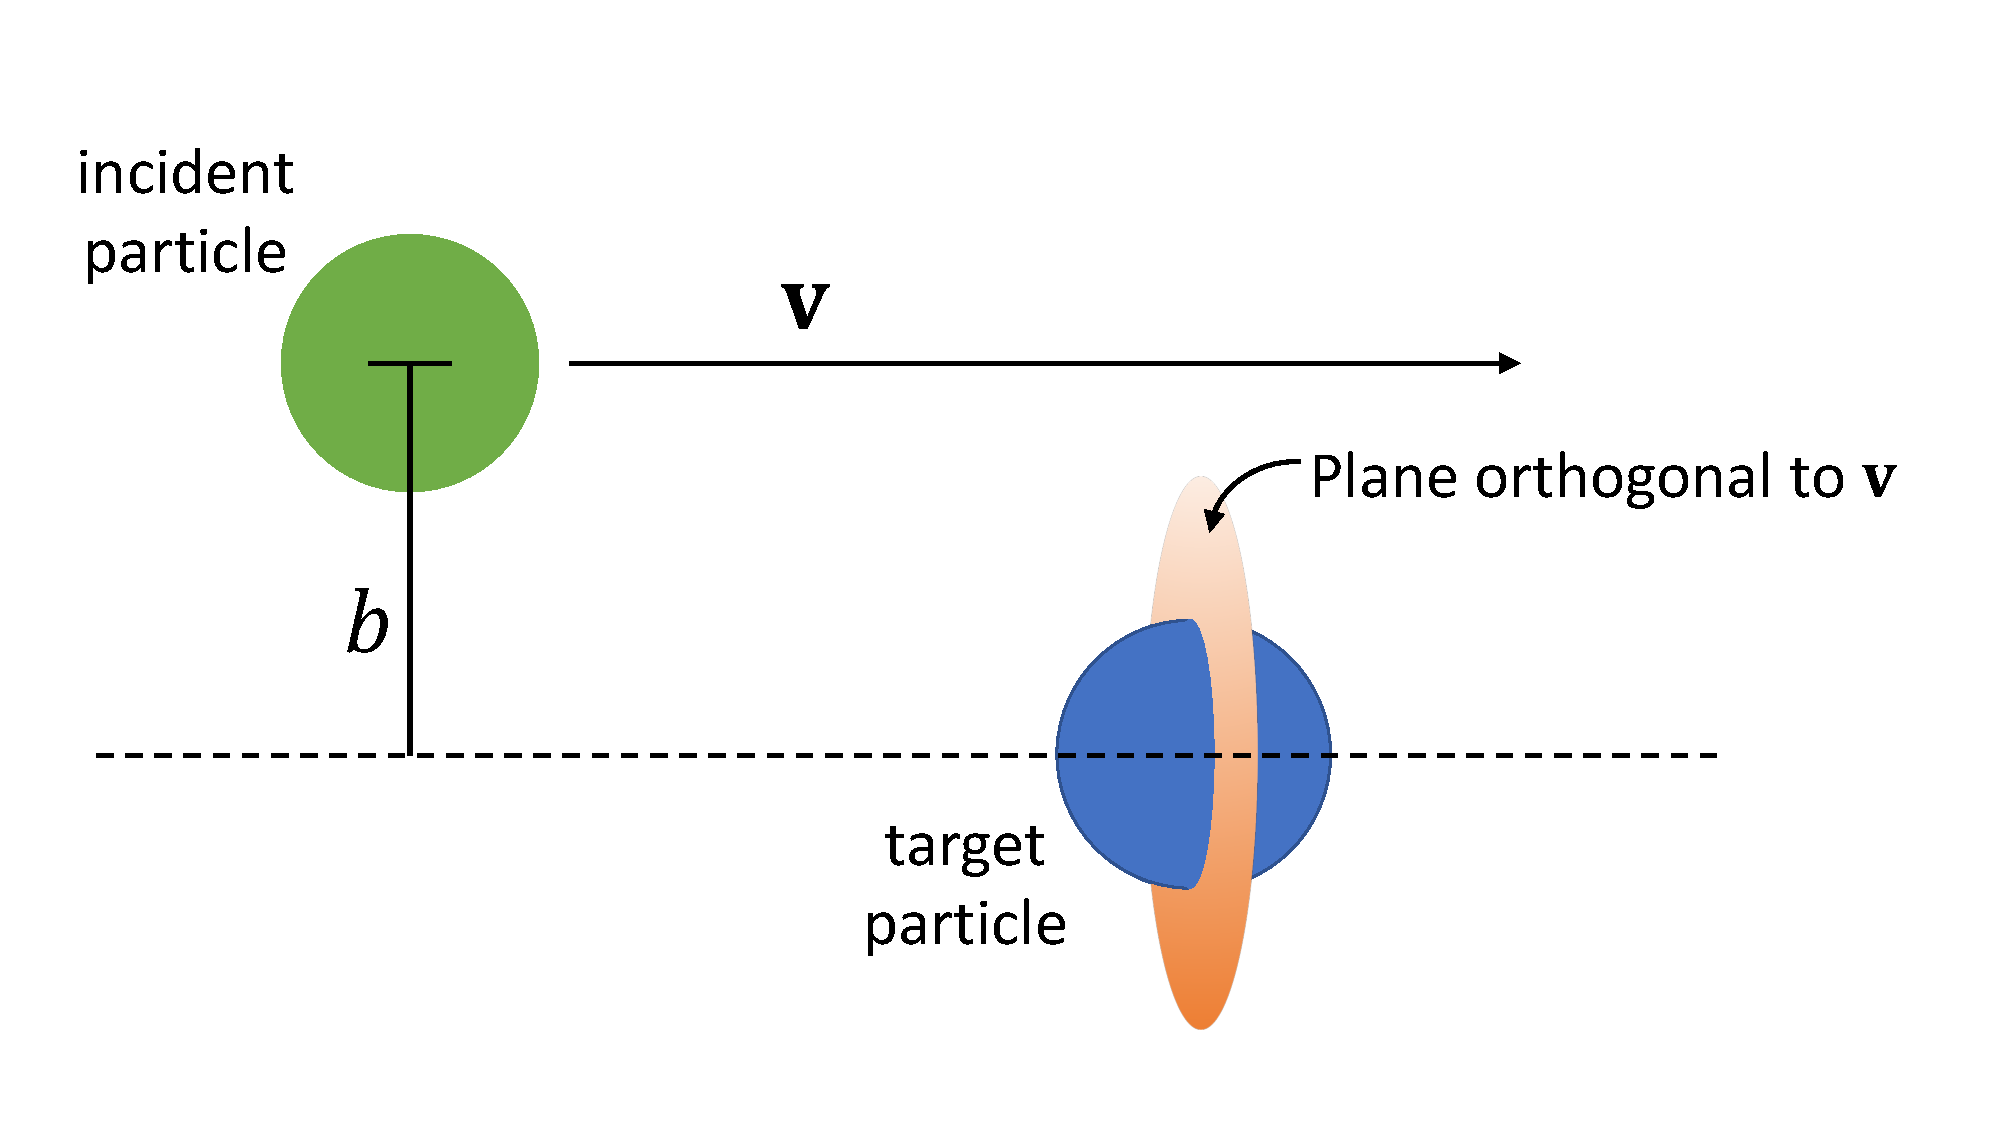
\includegraphics[width=10cm]{../../images/cross_section.pdf}
    \caption{Interaction of incident and target particles.}
    \label{fig:cross_many_particles}
\end{figure}
To define the cross section, we'll consider $I$ incident particles heading towards $J$ stationary target particles (see \cref{fig:cross_many_particles}). Not all of the incident particles will interact with the target particles, some will instead continue to travel in a uniform trajectory. The number of incident particles that do interact with the target particles is labeled as $N$. The cross section $\sigma$ is then a constant of proportionality defined by the following equation
\begin{equation}
    \label{eq:cross_def}
    N = \sigma I n_A.
\end{equation}
In the above, $n_A$ is the areal number density, that is, $n_A = J / A = n \Delta x$, where $n$ is the volume number density.

%-------------------------------------------------------------------------
\section{Differential cross section}
%-------------------------------------------------------------------------
\begin{figure}[ht]
    \centering
    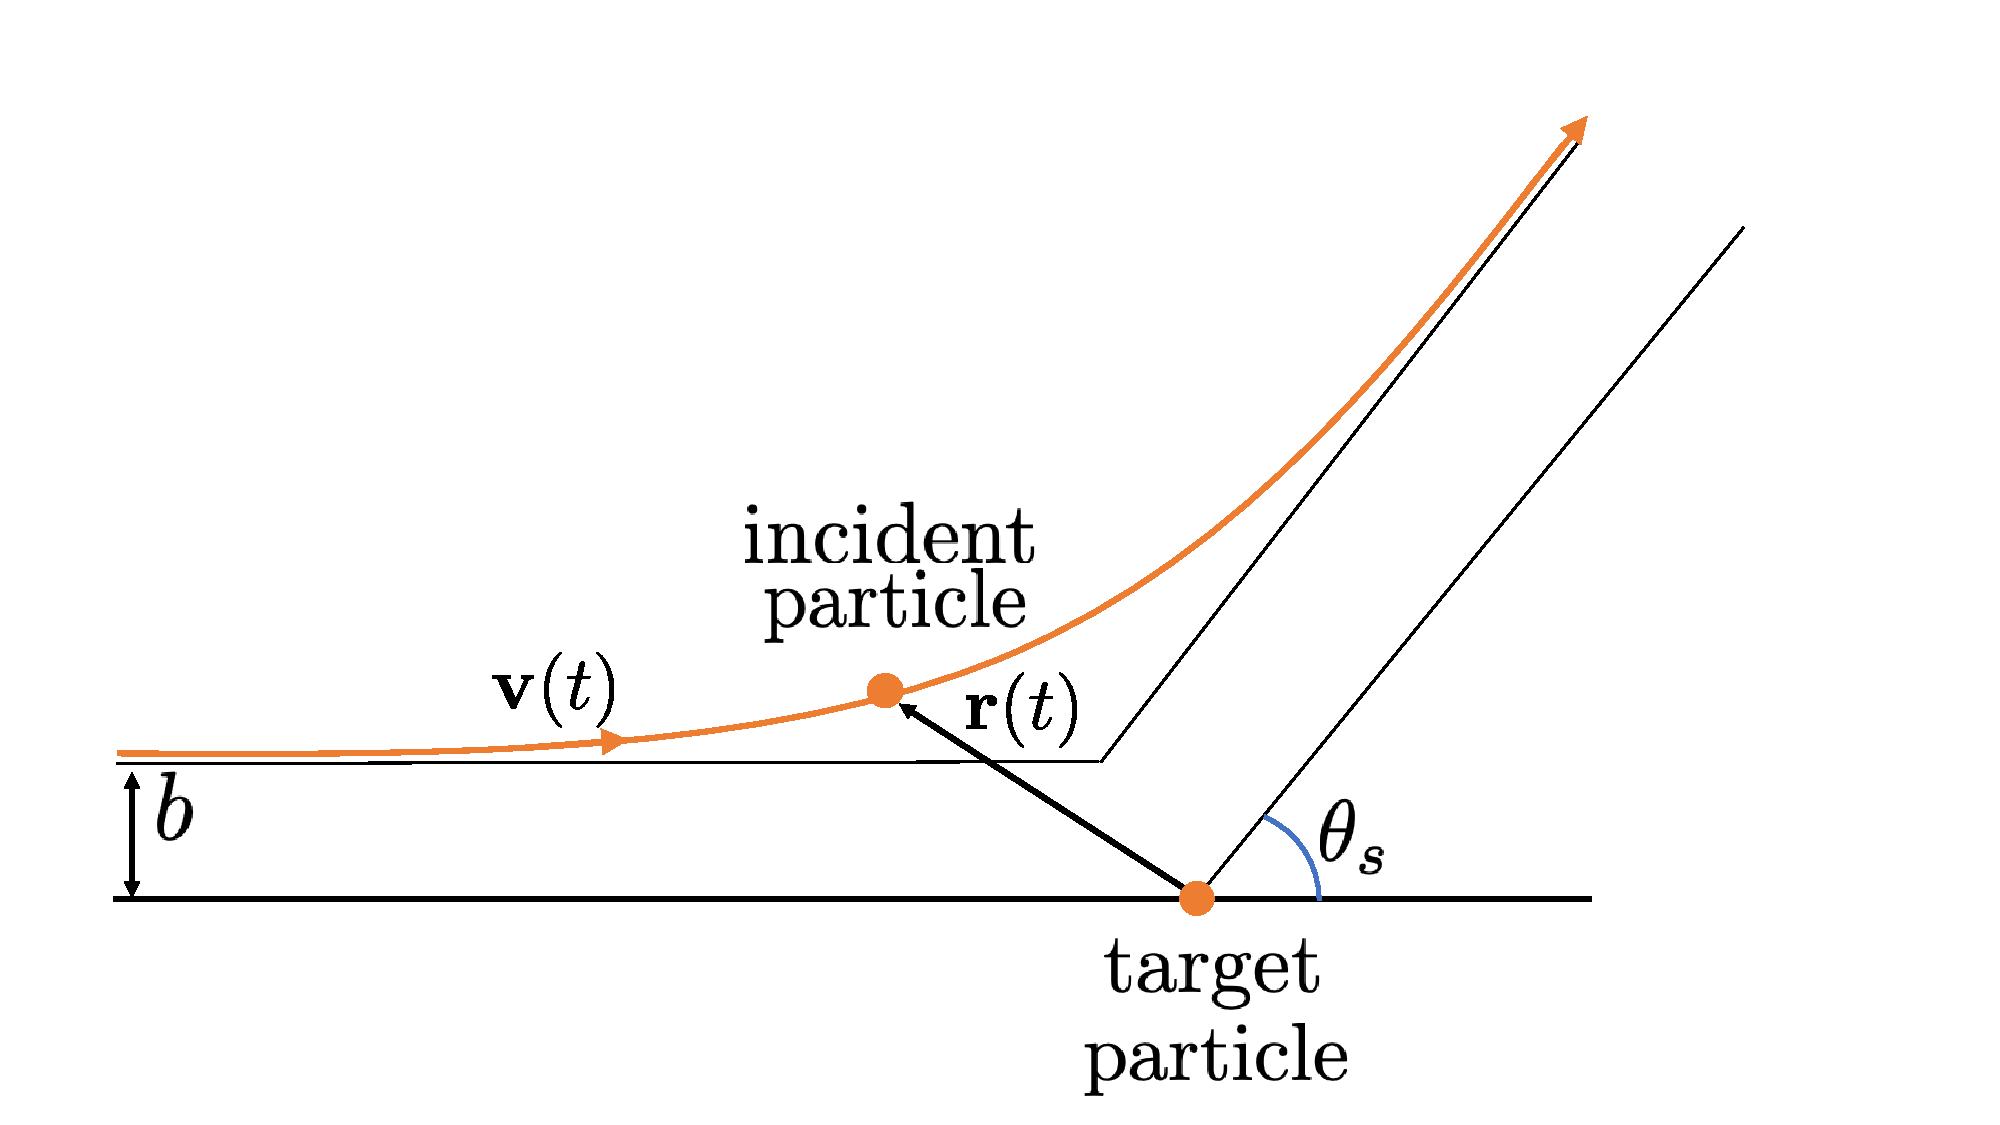
\includegraphics[width=10cm]{../../images/scattering.pdf}
    \caption{Depiction of particle scattering.}
    \label{fig:scattering}
\end{figure}

Consider the scattering of two particles: an incident and a target particle. If we fix the reference frame to follow the target particle, then the scattering can be depicted as shown in \cref{fig:scattering}. The displacement parameter is labelled as $b$, and the scattering angle as $\theta_s$. For three dimensional scattering, the encounter is as shown in \cref{fig:scattering_3d}. Not that in that figure the incident particle starts within the $x-z$ plane, and after scattering the particle is confined to a plane that is tilted an angle $\phi_s$ from the $x-z$ plane.

\begin{figure}[ht]
    \centering
    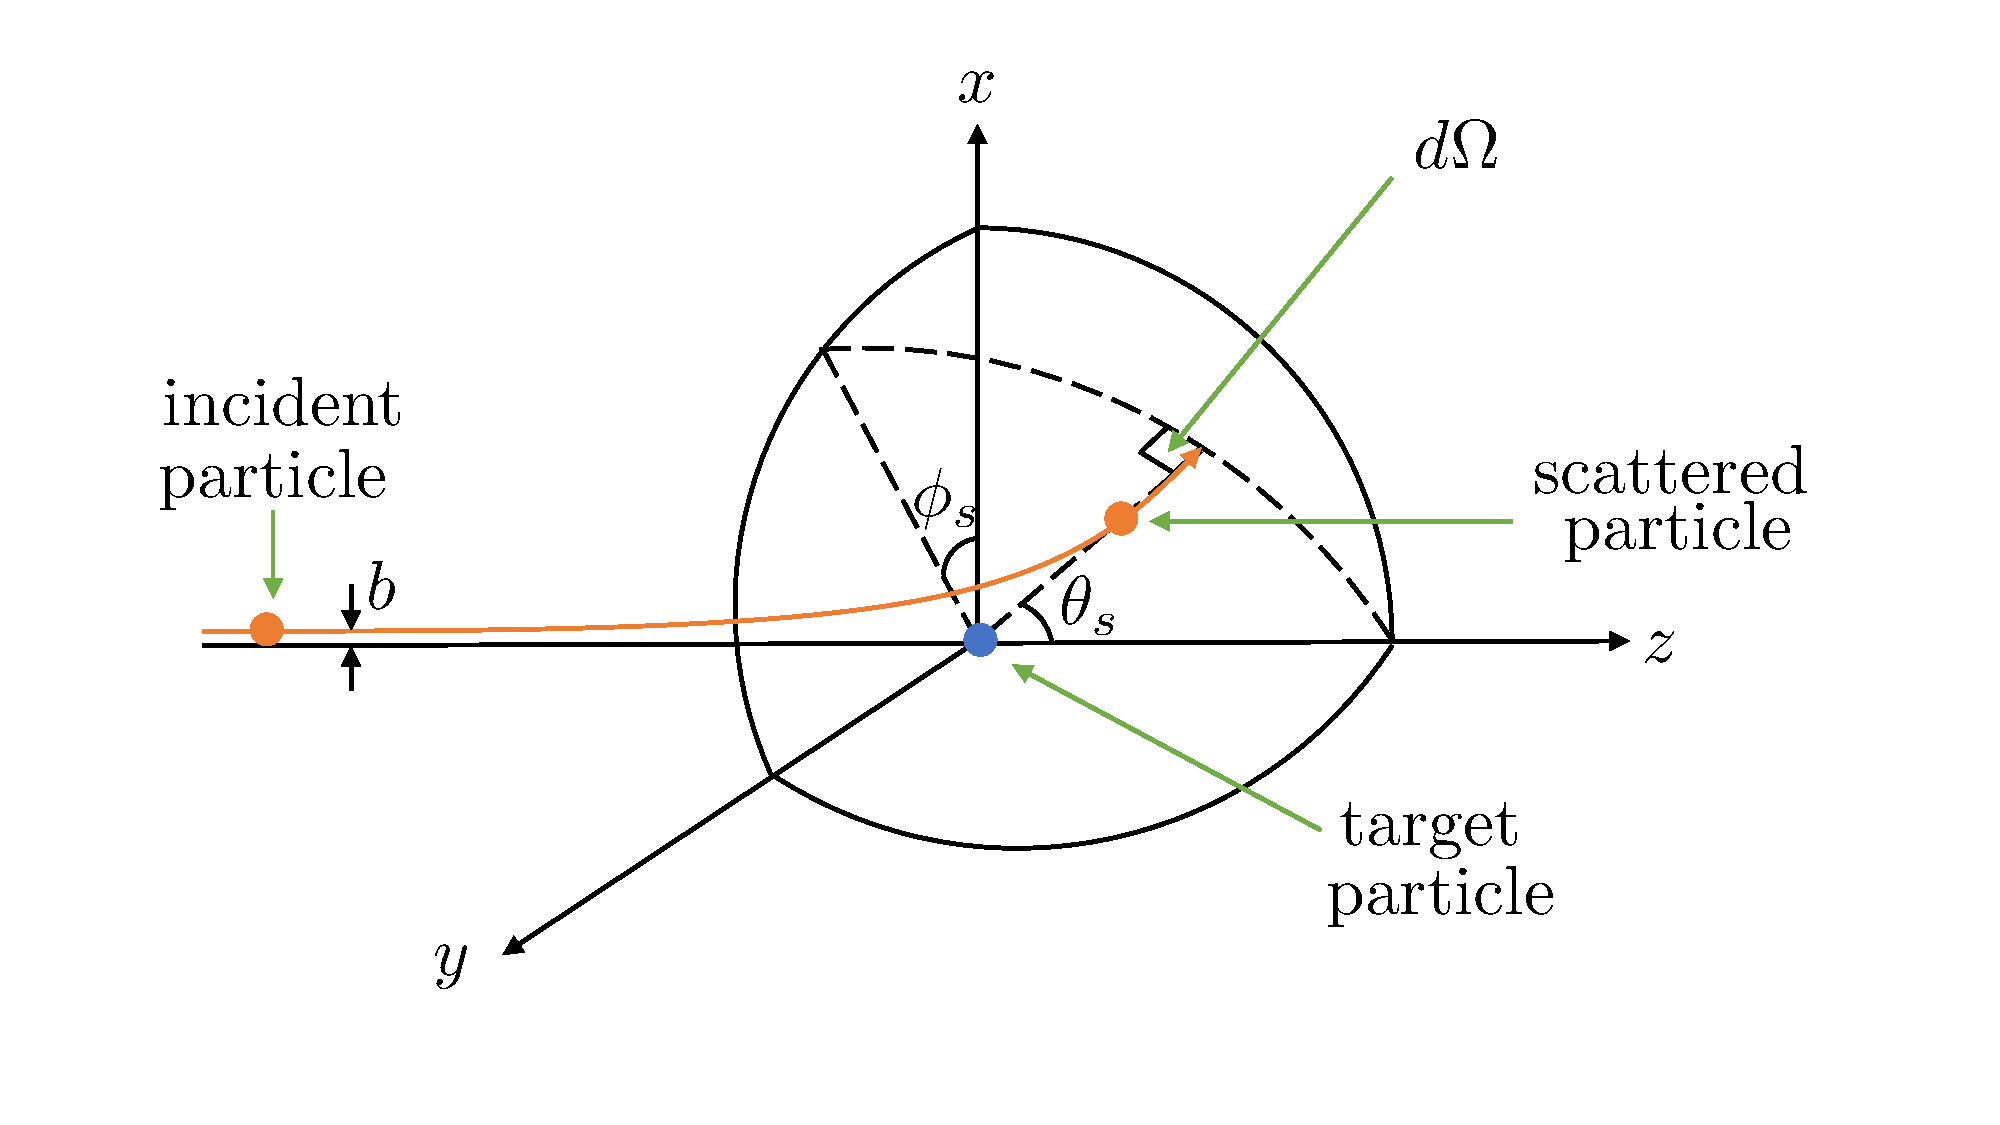
\includegraphics[width=10cm]{../../images/scattering_3d.pdf}
    \caption{Depiction of particle scattering in 3D.}
    \label{fig:scattering_3d}
\end{figure}

From the entire set of incident particles $N$ that interact with the target particles, one can define an infinitesimal subset $N_{\theta,\phi} d\Omega$ as the number of particles scattered into an infinitesimal solid angle $d\Omega = \sin \theta_s d\theta_s d\phi_s$, as shown in \cref{fig:scattering_3d}. We note that $N_{\theta,\phi} = N_{\theta,\phi} (\theta_s, \phi_s)$. The subset of particles $N_{\theta, \phi} d\Omega$ is now given by
\begin{equation}
    \label{eq:cross_def_diff}
    N_{\theta, \phi} d\Omega = \left ( \frac{d\sigma_{\theta,\phi}}{d\Omega} d\Omega \right ) I n_A.
\end{equation}
In the above, 
\begin{equation}
    \frac{d\sigma_{\theta,\phi}}{d\Omega} = \frac{d\sigma_{\theta,\phi}}{d\Omega}(\theta_s,\phi_s)
\end{equation}
is the differential cross section. It is best to not think of it as a derivative (what does a derivative with respect to solid angle mean?) and instead to simply think of it as a function that depends on $\theta_s$ and $\phi_s$. Integrating over all $\theta_s$ and $\phi_s$, i.e.
\begin{equation}
    \int_{\theta_s = 0}^\pi \int_{\phi_s = 0}^{2\pi} N_{\theta, \phi} d\Omega = \int_{\theta_s = 0}^\pi \int_{\phi_s = 0}^{2\pi} \frac{d\sigma_{\theta,\phi}}{d\Omega}  d\Omega I n_A
\end{equation}
gives \cref{eq:cross_def}.

\begin{figure}[ht]
    \centering
    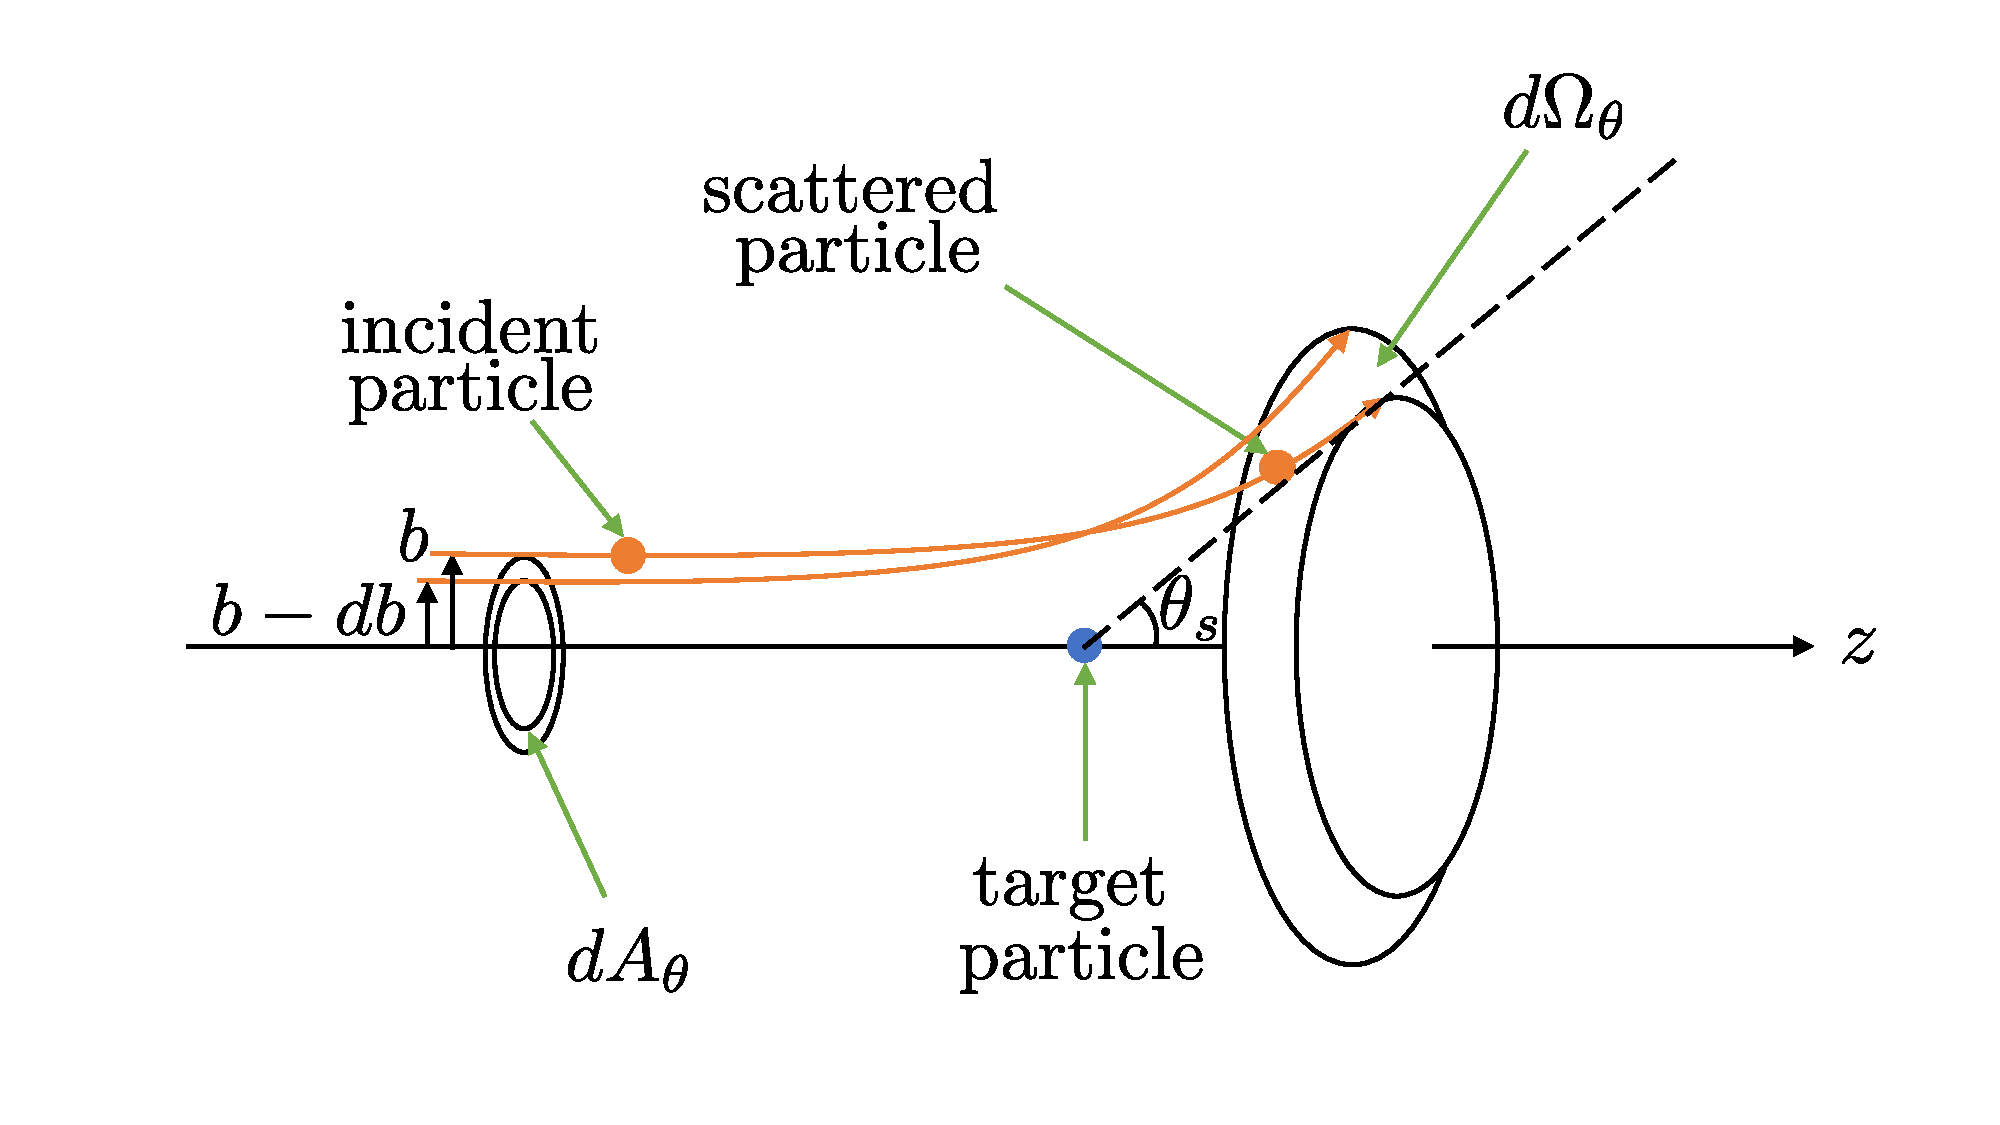
\includegraphics[width=10cm]{../../images/scattering_axi.pdf}
    \caption{Depiction of particle scattering in for axisymmetric interactions.}
    \label{fig:scattering_axi}
\end{figure}
For various cases the scattering is axisymmetric, that is, it is independent of $\phi_s$. Thus
\begin{equation}
    N_{\theta, \phi} \to N_\theta \qquad \frac{d\sigma_{\theta,\phi}}{d\Omega} \to \frac{d\sigma_\theta}{d\Omega},
\end{equation}
where 
\begin{equation}
    N_\theta = N_\theta (\theta_s),
\end{equation}
and
\begin{equation}
    \frac{d\sigma_\theta}{d\Omega} = \frac{d\sigma_\theta}{d\Omega} (\theta_s).
\end{equation}
Integrating \cref{eq:cross_def_diff} from $\phi_s = 0$ to $\phi_s = 2\pi$ gives
\begin{equation}
    \label{eq:cross_def_diff_axi}
    N_\theta d\Omega_\theta = \frac{d\sigma_\theta}{d\Omega} d\Omega_\theta I n_A,
\end{equation}
where $d \Omega_\theta = 2\pi \sin \theta_s d\theta_s$. $N_\theta d\Omega_\theta$ thus represents the number of particles that are scattered into the infinitesimal band $d\Omega_\theta$ on a sphere, where $d\Omega_\theta$ is defined by scattering angle $\theta_s$ (see \cref{fig:scattering_axi}). We will note that there is a one-to-one correspondence between the impact parameter $b$ and the scattering angle $\theta_s$, that is, $b = b(\theta_s)$. Thus, any incident particle scattered out through the infinitesimal band $d\Omega_\theta$ would have approached the target-particle through the infinitesimal ring $dA_\theta$ that corresponds to $d\Omega_\theta$. Since there are many target particles, there are many $dA_\theta$'s that correspond to the same $d\Omega_\theta$. Thus, the total number of particles scattered through $d\Omega_\theta$ is given by all the incident particles that cross through the $dA_\theta$'s of all the target particles.

The number of incident particles crossing all the infinitesimal rings $dA_\theta$ is equal to the total number of incident particles $I$ times the probability $P$ that a single incident particle will cross one of those rings. Thus, we can write
\begin{equation*}
    N_\theta d\Omega_\theta = I P.
\end{equation*}
The probability that an incident particle will cross one of those rings is simply the ratio of the surface area covered by all the rings in a section of the target material to the total area of that section. The surface area covered by all the rings in a section of area $S$ is given by $(n_A S) dA_\theta$. Thus, $P = n_A dA_\theta$ and 
\begin{equation*}
    N_\theta d\Omega_\theta = I n_A dA_\theta.
\end{equation*}
We now introduce the differential 
\begin{equation}
    \label{eq:cross_impact_differential}
    db = \frac{db}{d\theta_s} d\theta_s.
\end{equation}
We note that by definition $d\theta_s$ is positive but $db$ can be either positive or negative depending on the sign of $db/d\theta_s$. The infinitesimal area $dA_\theta$ is then given by 
\begin{equation}
    \label{eq:cross_impact_area}
    dA_\theta= 2\pi b |db| = 2 \pi b \left | \frac{db}{d\theta_s} \right | d \theta_s.
\end{equation}
Thus, 
\begin{equation*}
    N_\theta d\Omega_\theta = n_A I 2 \pi b \left | \frac{db}{d\theta_s} \right | d \theta_s.
\end{equation*}
Using \cref{eq:cross_def_diff_axi} in the above, we get
\begin{equation*}
    \frac{d\sigma_\theta}{d\Omega} d\Omega_\theta I n_A = I n_A 2 \pi b \left | \frac{db}{d\theta_s} \right | d \theta_s, 
\end{equation*}
or 
\begin{equation}
    \label{eq:cross_diff_impact_axi}
    \frac{d\sigma_\theta}{d\Omega} = \frac{b}{\sin \theta_s} \left | \frac{db}{d\theta_s} \right |.
\end{equation}

%-------------------------------------------------------------------------
\section{Mean free path \& collision frequency}
%-------------------------------------------------------------------------
The mean free path can be expressed in terms of the cross section as
\begin{equation}
    \lambda_m = \frac{1}{n_1 \sigma}.
\end{equation}
Given the particle's speed $v$, on can also define the collision time as follows
\begin{equation}
    \tau_m = \frac{\lambda_m}{v} = \frac{1}{n_1 \sigma v}.
\end{equation}
Finally, the collision frequency is simply the inverse of the collision time, that is
\begin{equation}
    \nu_{m} = \frac{1}{\tau_m} = n_1 \sigma v.
\end{equation}

%-------------------------------------------------------------------------
\section{The coupling parameter}
%-------------------------------------------------------------------------

Coulomb interactions are those which occur when two charge particles head towards each other. We can define two types of Coulomb interactions: strong and weak. Strong Coulomb interactions are those for which the particle's Coulomb potential energy is larger than its kinetic energy, and viceversa for weak Coulomb interactions. Thus, we can also define two types of plasma regimes:
\begin{itemize}
    \item Strongly-coupled plasmas: plasmas where the Coulomb interactions are mostly strong and thus drive the dynamics of its evolution. Coulomb interactions tend to be strong when the inter-particle distances are small, and thus this regime would be dominated by \textit{short-range} interactions. These plasmas are also described as exhibiting \textit{collisional} behavior, since a strong Coulomb interaction essentially means a collision has occurred.
    \item Weakly-coupled plasmas: plasmas where the Coulomb interactions are mostly weak, and as a result do not drive the dynamics of its evolution. The plasma dynamics are instead driven by \textit{long-range} effects caused by smooth electromagnetic fields that result from integrating a large number of particles. These plasmas are also described as exhibiting \textit{collective} behavior, since the long-range electromagnetic fields follow from the collective integration of many particles.
\end{itemize}

We describe an approximate Coulomb potential energy for particles in a plasma as
\begin{equation}
    U =  \frac{q_\alpha^2}{4 \pi \epsilon_0 a_\alpha}.
\end{equation}
The impact parameter that has been used above is $a_\alpha$, the sphere radius. This provides a decent measure on the average spacing between particles in a plasma. Since the volume of a single particle is $1/n_\alpha$, and if we assume that this volume is given by $4/3 \pi a_\alpha^3$, then equating these two gives the expression for the sphere radius
\begin{equation}
    a_\alpha = \left ( \frac{3}{4 \pi n_\alpha} \right )^{1/3}.
\end{equation}
The thermal velocity of a particle is given by
\begin{equation}
    v_{T_\alpha} = \sqrt{\frac{k_B T_\alpha}{m_\alpha}}
\end{equation}
A measure of the kinetic energy of a particle is given in terms of the thermal velocity as shown below
\begin{equation}
    K = m_\alpha v_{T_\alpha}^2 = k_B T_\alpha
\end{equation}
The ratio of the particle's Coulomb potential energy and its kinetic energy is referred to as the coupling parameter $\Gamma_\alpha$. That is 
\begin{equation}
    \Gamma_\alpha = \frac{q_\alpha^2}{4 \pi \epsilon_0 a_\alpha k_B T_\alpha}.
\end{equation}
$\Gamma_\alpha > 1$ denotes a strongly coupled plasma, and $\Gamma_\alpha < 1$ denotes a weakly coupled plasma. 

%-------------------------------------------------------------------------
\section{The plasma parameter}
%-------------------------------------------------------------------------
The standard plasma parameter $\Lambda_\alpha$ is defined as
\begin{equation}
    \Lambda_\alpha = \frac{4}{3} \pi \lambda_{D\alpha}^3 n_\alpha.
\end{equation}

There is a one to one relationship between the coupling parameter and the standard plasma parameter. Simple algebra shows that 
\begin{equation}
    \Gamma_\alpha = (1/3) \Lambda_\alpha^{-2/3}.
\end{equation}
Thus, the coupling and plasma parameters are inversely proportional to each other. $\Lambda_\alpha < 1$ implies strongly-coupled plasmas, and $\Lambda_\alpha > 1$ weakly-coupled plasmas. Since $\Lambda_\alpha$ represents the number of particles per Debye sphere, it is interesting to see that a large number of particles within such a sphere is needed to be in the weakly-coupled-plasma regime. However, this does not correspond to a plasma with large density, in fact, it corresponds to the opposite. The explicit $n_\alpha$ term in the definition $\Lambda_\alpha = (4/3) \pi \lambda^3_{D\alpha} n_\alpha$ is dominated by the $n_\alpha$ in the denominator of $\lambda_{D\alpha}$. In other words, low plasma densities lead to large Debye spheres, which in turn leads to many particles per Debye sphere, and hence a weakly-coupled plasma.

%-------------------------------------------------------------------------
\section{Electron degeneracy}
%-------------------------------------------------------------------------

\begin{itemize}
    \item DeBroglie wavelength
    \begin{equation}
        \lambda_{B\alpha} = \dfrac{h}{\sqrt{2 \pi} m_\alpha v_{T\alpha}}
    \end{equation}
    \item Quantum plasma parameter
    \begin{equation}
        \chi_\alpha = \frac{4}{3} \pi \lambda_{B\alpha}^3 n_\alpha
    \end{equation}
    
    \item Fermi energy:
    \begin{equation}
        E_{f\alpha} = \frac{\hbar^2}{2m_\alpha} \left ( 3 \pi^2 n_\alpha \right)^{2/3}
    \end{equation}

    \item The Fermi energy can be used to define the Fermi temperature $T_{f\alpha}$, Fermi velocity $v_{f\alpha}$, Fermi momentum $p_{f\alpha}$, and Fermi wavevector $k_{f\alpha}$
    \begin{equation}
        E_{f\alpha} = k_B T_{f\alpha} = \frac{1}{2} m_\alpha v_{f\alpha}^2  = \frac{p_{f\alpha}^2}{2m_\alpha} = \frac{\left ( \hbar k_{f\alpha} \right ) ^2}{2m_\alpha}
    \end{equation}

    \item Degeneracy parameter:
    \begin{equation}
        \Theta_\alpha = \frac{k_B T_\alpha}{E_{f\alpha}} = \left( \frac{2^{10} \pi}{3^4} \right)^{1/3} \chi_\alpha^{-2/3}
    \end{equation}
\end{itemize}

\bibliographystyle{plainnat}
\bibliography{library}
\end{document}
